\begin{figure}[!tb]
\begin{center}
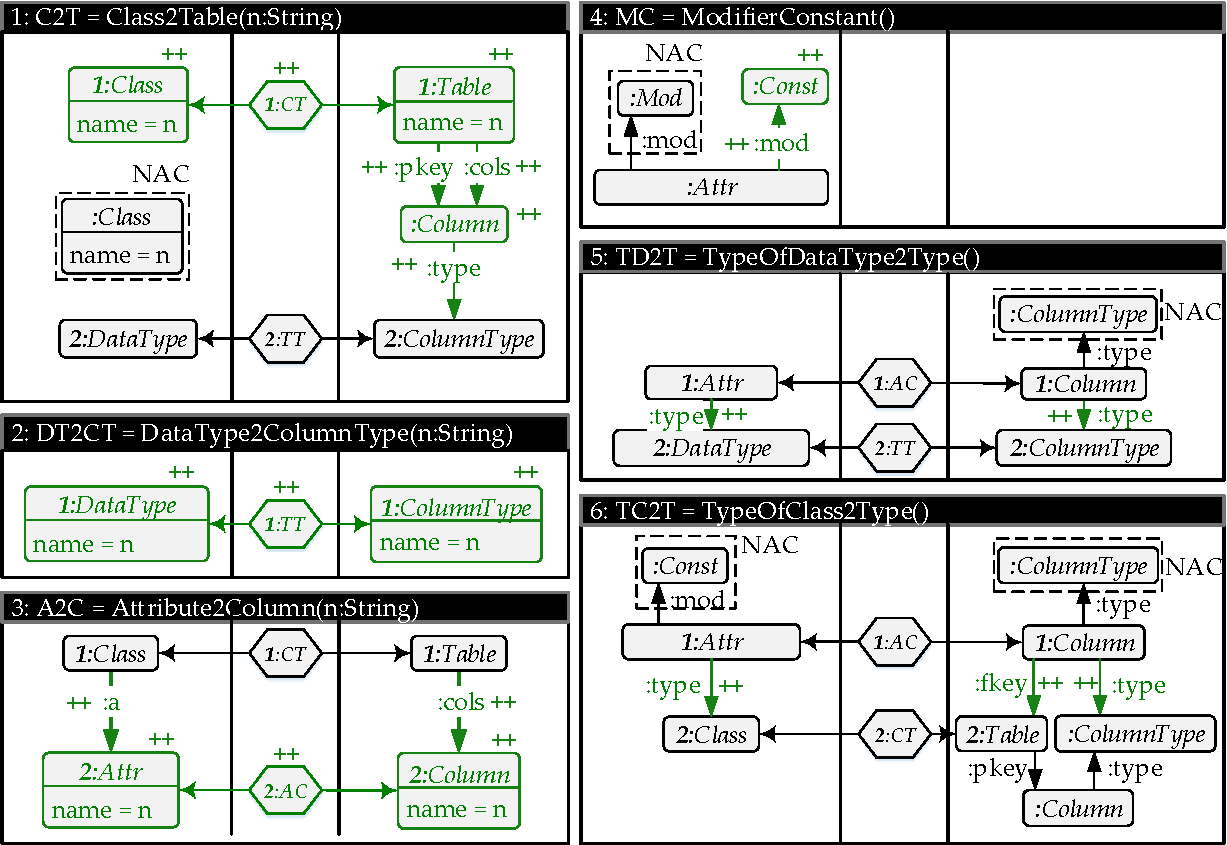
\includegraphics[width=\textwidth]{img/gen_intro/tgg.pdf}
\end{center}
\caption{Triple Graph Grammar (CD2RDBM)}
\label{fig:sec-gt-trafo:tgg}
\label{fig:rules}
\end{figure}

As discussed in \cref{sec-gen-intro-gratrafo}, models are represented by graphs and model transformations and synchronisations are performed based on graph transformations.
Furthermore, graph transformations are performed by applying graph transformation rules to graphs.
According to \cref{def:sec-gt-trafo:rule}, a rule $p$ is a span $p=(L \transB{L} K \trans{r} R)$ of $\M$-morphisms $l$ and $r$ with left-hand side $L$, gluing $K$ and right-hand side $R$.
A rule is applied to a graph $G$ via a match-morphism $m\colon L \to G$ as defined by direct transformations in \cref{def:sec-gt-trafo:trafo}.

\begin{definition}[(Transformation) Rule (Def. 5.12 in \cite{FAGT2})]
\label{def:sec-gt-trafo:rule}
A \emph{plain (transformation) rule $p=(L \transB{l} K \trans{r} R)$}\index{transformation!rule!plain} consists of objects $L,K$ and $R$, called left-hand side, gluing and right-hand side, respectively and two morphisms $l,r \in \M$.
A \emph{(transformation) rule $p=(L \transB{l} K \trans{r} R, \ac_L)$}\index{transformation!rule} consists of a plain rule and a condition $\ac_L$ over $L$, called application condition.\index{application condition}
\envEndMarker
\end{definition}

\parpic[r][r]{
$
\SelectTips{cm}{}
     \xymatrix@R-3.3ex@C-2ex{
     L \ar[dd]|{m} & & K \ar[ll]|{l} \ar[rr]|{r} \ar[dd]|{k} & & R \ar[dd]|{n} \\
     & (1) & & (2) & \\
     G & & D \ar[ll]|{f} \ar[rr]|{g} & & H\\
     }
$
}
\vspace{-1.5ex}
\begin{definition}[Transformation (Def. 5.13 in \cite{FAGT2})]
\label{def:sec-gt-trafo:trafo}
Given a rule $p=(L \transB{l} K \trans{r} R, \ac_L)$, an object $G$, and a morphism $m\colon L \to G$, called match, such that $m \models \ac_L$, \emph{a direct transformation (step) $G \Trans{(p,m)} H$}\index{transformation!direct} from $G$ to an object $H$ via $p$ and match $m$ is given by the pushouts $(1)$ and $(2)$ with co-match $n$\index{match}\index{co-match}.
Given a set of rules $P$, a sequence of direct transformations from $G$ to $H$ via $p \in P$ is called \emph{a transformation (sequence) via $P$}\index{transformation}, written $t\colon G \Trans{*} H$.
\envEndMarker
\end{definition}

Intuitively, the application leads to a graph $H$ where $m(L) \setminus m(l(K))$ is deleted from $G$ and $R \setminus r(K)$ is added while $m(l(K))$ is preserved.
Furthermore, a rule may be equipped with an application condition $\ac_L$ which may restrict the application of the rule to specific matches, i.e, for rule applications, match $m$ must additionally satisfy application condition $\ac_L$.
According to \cref{def:sec-gc-gc:cond_pos}, we distinguish between positive application conditions (PACs) and negative application conditions (NACs)\index{application condition!NAC}\index{application condition!PAC}.
NACs declare forbidden patterns and PACs declare patterns that must exist for rule applications.
We say that a \emph{rule is non-deleting}\index{transformation!rule!non-deleting}, if $l=\id_L$ and $K=L$.
In case of non-deleting rules $p=(L \transB{id} L \xhookrightarrow{r} R,\ac_L)$, we write $p=(L \xhookrightarrow{r} R,\ac_L)$ and pushout $(1)$ in \cref{def:sec-gt-trafo:trafo} is omitted with $D=G$ and $k=m$.
According to \cref{sec-gt-graphs,def:sec-gt-graphs:typed_graphs} and \cref{sec-gt-gc,def:condition-satisfaction}, we say that a rule $p=(L \gets K \to R,\ac_L)$ is typed over type graph $\TG$\index{transformation!rule!typed over}, if $L,K,R$ and $\ac_L$ are typed over common $\TG$.
We take production as synonym for rule\index{production}.

A transformation system is a set of rules.
A transformation system together with a start object constitutes a grammar.
Usually, we take graphs as objects and speak of graph grammars (cf. \cref{sec-gt-M-adh,rem:sec-gt-M-adh}).
The language over a grammar is given by all objects that are reachable from the start object by transformations via the rules of the grammar (cf. \cref{sec-dc-general,def:sec-dc-general:lang}).
We say that a grammar is non-deleting\index{grammar!non-deleting}, if all its rules are non-deleting.
We say that a grammar is typed over $\TG$\index{grammar!typed over}, if the start object and all its rules are typed over $\TG$.
We say that a grammar is without application conditions, if all its rules are plain rules.
A grammar is finite\index{grammar!finite}, if the set of rules is finite.

\begin{definition}[$\M$-adhesive Transformation System \& Grammar]
\label{def:sec-gt-trafo:grammar}
Given an $\M$-adhesive categoriy $(\cat{C},\M)$, \emph{an $\M$-adhesive transformation system $\AS=(P)$}\index{transformation!system} is given by a set of rules $P$.
\emph{A grammar $\GG=(S,\AS)$}\index{grammar} is given by a transformation system $\AS$ and a start object $S$.
\envEndMarker
\end{definition}

\paragraph*{Visual Notation}
\label{par:sec-gt-trafo:vis_not}
In addition to the notational conventions from \cref{par:sec-gt-graphs:vis}, transformation rules are visualised as depicted in \cref{fig:sec-gt-trafo:tgg}.
All graph elements that are marked with \code{++} are added by the rule and therefore, are only contained in the right-hand side of the rule.
All graph elements that are marked with \code{--} are deleted by the rule and therefore, are only contained in the left-hand side of the rule.
All graph elements that are unmarked are preserved by the rule and therefore, are contained in the left-hand side and the gluing of the rule.
Additionally, a rule may be equipped with an application condition which consists of the left-hand side of the rule together with those graph elements that are enclosed by PAC or NAC boxes.

\begin{example}[Rules \& Transformations]
\label{ex:sec-gt-trafo:trafo}
The rules in \cref{fig:sec-gt-trafo:tgg} simultaneously create class diagrams and relational database models.
For each rule $p$, we focus on the projection $p^\SRC$ to the source domain of class diagrams (left parts).
Rule \code{1}$^\SRC$ creates a \code{Class} of \code{name} \code{n} in addition to an existing \code{DataType} but only of there does not already exist a class of the same name (cf. NAC).
Rule \code{2}$^\SRC$ creates a \code{DataType} of \code{name} \code{n}.
Rule \code{3}$^\SRC$ creates an \code{Attribute} of \code{name} \code{n} and assigns it to an existing \code{Class} via edge \code{:a}.
Rule \code{4}$^\SRC$ creates a \code{Const}ant \code{Mod}ifier to an existing attribute but only of the attribute does not already have a modifier (cf. NAC).
Rule \code{5}$^\SRC$ assigns an existing data type to an existing attribute as \code{type}.
Rule \code{6}$^\SRC$ assigns an existing class to an existing attribute as \code{type} but only if the attribute is not \code{Const}ant (cf. NAC).
There is a transformation $\varnothing \Trans{(\code{2}^\SRC,\_)} G_1 \Trans{(\code{1}^\SRC,\_)} G_2 \Trans{(\code{3}^\SRC,\_)} G_3 \Trans{(\code{4}^\SRC,\_)} G_4 \Trans{(\code{5}^\SRC,\_)} \CD$ from the empty graph $\varnothing$ to graph $\CD$ in \cref{sec-gt-graphs,fig:sec-gt-graphs:atg}.
Analogously, we derive six rules by a projection to the right parts that create the elements of relational database models.
\envEndMarker
\end{example}

In view of \cref{sec-dc-general-rec}, we recall the notion of the derived span of transformations.

\begin{definition}[Derived Span \cite{FAGT2}]
\label{def:sec-gt-trafo:derived_span}
Let $t\colon G_0 \Trans{*} G_n$ be a transformation, then the \emph{derived span $\der(t)$ of $t$}\index{transformation!derived span} is inductively defined by
\begin{center}
	$\der(t)=\begin{cases}
	G \transB{\id_G} G \trans{\id_G} G & ,\text{for identical (empty) transformation } t\colon G \Trans{\id} G \\
	G_{i-1} \transB{f_i} D_i \trans{g_i} G_i & ,\text{for }t\colon G_{i-1} \Trans{(p_i,m_i)} G_i \text{ being a direct transformation}\\
	& \text{with pushouts} (1) \text{ and } (2)\\
	G_0 \transB{d'_0 \circ d} D \trans{g_n \circ d_n} G_n & ,\text{for }t\colon G_0 \Trans{*} G_{n-1} \Trans{(p_n,m_m)} G_n \text{ with }\\
	& \der(G_0 \Trans{*} G_{n-1})=(G_0 \transB{d'_0} D' \trans{d'_{n-1}} G_{n-1})\\
	& \text{ and pullback }(PB)
	\end{cases}$
\end{center}
\envEndMarker
\begin{center}
	%\vspace*{.2cm}
	\begin{tikzpicture}[]
	\fill (0,0) node[inner sep=1pt] (G0) {$G_0$};
	\fill (0,0) node[right of=G0,xshift=1cm,inner sep=1pt] (D') {$D'$};
	\fill (0,0) node[right of=D',xshift=1cm,inner sep=1pt] (Gn1) {$G_{n-1}$};
	\fill (0,0) node[right of=Gn1,xshift=1cm,inner sep=1pt] (Dn) {$D_n$};
	\fill (0,0) node[right of=Dn,xshift=1cm,inner sep=1pt] (Gn) {$G_n$};
	\fill (0,0) node[below of=Gn1,yshift=-1cm,inner sep=1pt] (D) {$D$};
	%
	\fill (0,0) node[below of=Gn1,inner sep=1pt] (1) {$(PB)$};
	%
	\fill (0,0) node[left of=G0,xshift=-4cm,inner sep=1pt] (Lp) {$L_i$};
	\fill (0,0) node[right of=Lp,xshift=.5cm,inner sep=1pt] (Kp) {$K_i$};
	\fill (0,0) node[right of=Kp,xshift=.5cm,inner sep=1pt] (Rp) {$R_i$};
	\fill (0,0) node[below of=Lp,yshift=-1cm,inner sep=1pt] (G0p) {$G_{i-1}$};
	\fill (0,0) node[right of=G0p,xshift=.5cm,inner sep=1pt] (D1p) {$D_i$};
	\fill (0,0) node[right of=D1p,xshift=.5cm,inner sep=1pt] (G1p) {$G_i$};
	%
	\fill (0,0) node[left of=Lp,xshift=.3cm,inner sep=1pt] (p1) {$p_i=($};
	\fill (0,0) node[right of=Rp,xshift=-.7cm,inner sep=1pt] (p2) {$)$};
	\fill (0,0) node[right of=Lp,xshift=-.25cm,yshift=-1cm,inner sep=1pt] (1) {$(1)$};
	\fill (0,0) node[right of=Lp,xshift=1.25cm,yshift=-1cm,inner sep=1pt] (2) {$(2)$};
	%
	{
	\pgfsetarrows{right hook-latex}
	%
	\pgfsetarrows{left hook-latex}
	%
	\pgfsetarrows{-latex}
	\path (D') edge[] node[fill=white]{\scriptsize{$d'_0$}} (G0);
	\path (D') edge[] node[fill=white]{\scriptsize{$d'_{n-1}$}} (Gn1);
	\path (Dn) edge[] node[fill=white]{\scriptsize{$f_n$}} (Gn1);
	\path (Dn) edge[] node[fill=white]{\scriptsize{$g_n$}} (Gn);
	\path (D) edge[] node[fill=white]{\scriptsize{$d$}} (D');
	\path (D) edge[] node[fill=white]{\scriptsize{$d_n$}} (Dn);
	%
	\path (Kp) edge[] node[fill=white]{\scriptsize{$l_i$}} (Lp);
	\path (Kp) edge[] node[fill=white]{\scriptsize{$r_i$}} (Rp);
	\path (D1p) edge[] node[fill=white]{\scriptsize{$f_i$}} (G0p);
	\path (D1p) edge[] node[fill=white]{\scriptsize{$g_i$}} (G1p);
	\path (Lp) edge[] node[fill=white]{\scriptsize{$m_i$}} (G0p);
	\path (Kp) edge[] node[]{} (D1p);
	\path (Rp) edge[] node[]{} (G1p);
	%
	\pgfsetarrows{->>}
	%
	}
	\end{tikzpicture}
\end{center}
\end{definition}

\begin{remark}[Derived Span for Non-Deleting Rules]
\label{rem:sec-gc-gc:der_span_non_deleting}
For transformations $t\colon G_0 \Trans{*} G_n$ via non-deleting rules only and with direct transformations $(G_{i-1} \Trans{(p_i,m_i)} G_i)_{i \in \{1,\ldots,n\}}$, the derived span $\der(t)\colon G_0 \to G_n$ of $t$ is given by $\der(t):=g_n \circ \ldots \circ g_1$.
Note that in $\M$-adhesive categories, the derived span for transformations via non-deleting productions is in $\M$ by productions being spans of $\M$-morphisms ($r_i \in \M$), $\M$-morphisms are closed under pushouts, i.e., $g_i \in \M$, and $\M$-composition, i.e., $g_n \circ \ldots \circ g_1 \in \M$.
\envEndMarker
\end{remark}

\parpic[r][r]{
$
\SelectTips{cm}{}
     \xymatrix@R-3.3ex@C-2ex{
     A \ar[dd]|{} \ar[rr]|{} & & B \ar[rr]|{} \ar[dd]|{} & & E \ar[dd]|{} \\
     & (1) & & (2) & \\
     C \ar[rr]|{} & & D \ar[rr]|{} & & F\\
     }
$
}
\vspace{-1.5ex}
We review the following general existing results, as, they are used in definitions or proofs:
\begin{enumerate*}
\item [\textbf{Restriction Theorem} (Thm. 6.18 in \cite{Ehrig:2006:FAG:1121741})]\index{restriction theorem}: Direct transformations can be restricted along specific decompositions of match-morphisms,
\item [\textbf{PO-(De)-Composition} (Lem. A.21 in \cite{Ehrig:2006:FAG:1121741})]\index{pushout!composition}\index{pushout!decomposition}: For pushouts $(1)$ and $(2)$, also $(1)+(2)$ is a pushout, and if $(1)$ and $(1)+(2)$ are pushouts, then also $(2)$, and
\item [\textbf{PB-(De)-Composition} (Lem. A.25 in \cite{Ehrig:2006:FAG:1121741})]\index{pullback!composition}\index{pullback!decomposition}: For pullbacks $(1)$ and $(2)$, also $(1)+(2)$ is a pullback, and if $(2)$ and $(1)+(2)$ are pullbacks, then also $(1)$.
\item [\textbf{Critical Pair}]\index{critical pair}: Given a transformation system $P$, a critical pair $(K_1 \TransB{(p_1,m_1)} O \Trans{(p_2,m_2)} K_2)$ for rules $P$ is a pair of direct transformations $t_1\colon O \Trans{(p_1,m_1)} K_1$ and $t_2\colon O \Trans{(p_2,m_2)} K_2$ with common object $O$ and $p_1,p_2 \in P$ where both transformations are in conflict to each other, intuitively, in the sense that
(1) transformation $t_1$ deletes elements from $O$ to $K_1$ that are ``used'' by match $m_2$ for transformation $t_2$ or vice versa, or
(2) $K_1$ does not satisfy the application condition of $p_2$ anymore or vice versa
and furthermore, where object $O$ is minimal.
Object $O$ is minimal means that matches $m_1$ and $m_2$ are jointly epimorphic (surjective) on $O$, i.e., $O$ only contains elements that are covered by transformations $t_1$ and $t_2$.
In the context of graphs, $O$ is called the conflict graph of the critical pair.\index{conflict graph}
For technical details we refer to Def. 2.39 in \cite{FAGT2}.
Note that we concentrate on critical pairs for rules over graphs with translation (marking) attributes (cf. \cref{sec-mt-tgg,rem:sec-mt-tgg:tr_attr}).
This involves forward translation rules (cf. \cref{sec-mt-tgg,def:sec-mt-tgg:fwd_bwd_tr_rules}), consistency creating rules (cf. \cref{sec-msynch-tgg,def:sec-msynch-tgg:cc_rule}) and marking rules (cf. \cref{sec-dc-verification,def:marking-rule}) that only update translation (marking) attributes from $\False$ to $\True$ while preserving the remaining graph structure in terms of deletions.
Note that technically, the update of an attribute is a deletion of the old attribute value followed by a creation of the new attribute value (cf. \cref{sec-gt-graphs,def:sec-gt-graphs:agraphs}).
\cref{fig:sec-gt-trafo:cp} depicts a critical pair $(K_1 \TransB{(m(4^S),m_1)} O \Trans{(m(4^S),m_2)} K_2)$ for marking rule $m(4^S)$ of rule $4^S$ in \cref{ex:sec-gt-trafo:trafo}.
Both transformations simultaneously update the marking attribute of node \code{1:Const} from $\False$ to $\True$.
\item [\textbf{Strict Confluence}]\index{critical pair!strict confluence}: A critical pair $(K_1 \TransB{(p_1,m_1)} O \Trans{(p_2,m_2)} K_2)$ is strictly confluent, if there are transformations $t_1\colon K_1 \Trans{*} O'$ and $t_2\colon K_2 \Trans{*} O'$ to common $O'$ such that all elements that are preserved by both transformations of the critical pair are also preserved by transformations $t_1$ and $t_2$ such that they can be embedded into bigger contexts.
For technical details we refer to Def. 2.42 in \cite{FAGT2}.
\item [\textbf{Local Confluence Theorem} (Thm. 2.43 in \cite{FAGT2})]\index{local confluence}\index{local confluence theorem}: A transformation system $P$ is locally confluent if, for all direct transformations $G \Trans{(p_1,m_1)} H_1$ and $G \Trans{(p_2,m_2)} H_2$ via $p_1,p_2 \in P$, there is an object $X$ and transformations $H_1 \Trans{*} X$ and $H_" \Trans{*} X$ via $P$.
A transformation system is locally confluent if all its critical pairs are strictly confluent.
\item [\textbf{Confluence} (Lem. 3.32 in \cite{Ehrig:2006:FAG:1121741})]\index{confluence}: A transformation system $P$ is confluent if, for all transformations $G \Trans{*} H_1$ and $G \Trans{*} H_2$ via $P$, there is an object $X$ and transformations $H_1 \Trans{*} X$ and $H_2 \Trans{*} X$ via $P$.
Every terminating and locally confluent transformation system is also confluent.
\index{transformation!system!terminating}A transformation system $P$ is terminating if there is no infinite transformation sequence via $P$.
\end{enumerate*}

\begin{figure}[!tb]
\begin{center}
	\begin{tikzpicture}[]
	\fill (0,0) node[inner sep=1pt] (P) {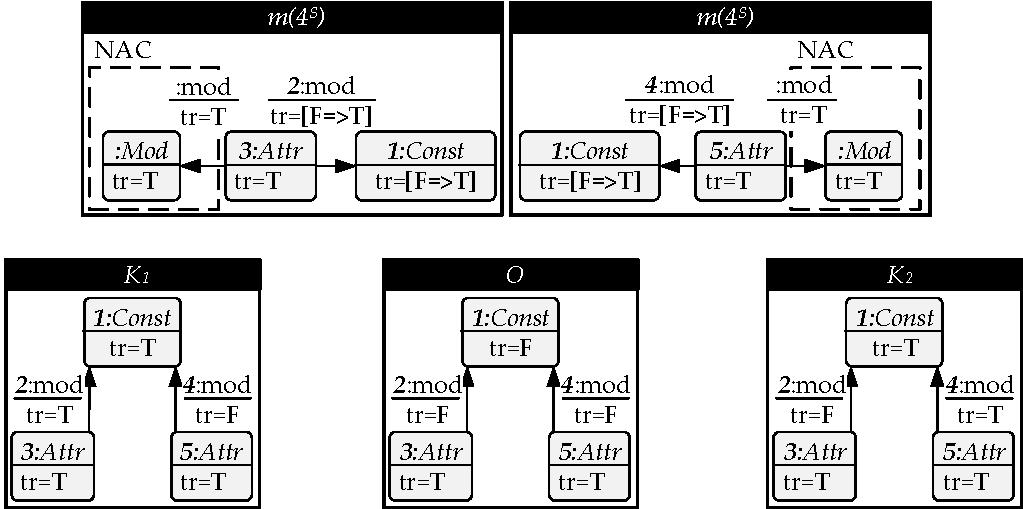
\includegraphics[width=.95\textwidth]{img/dc/cp.pdf}};
	\fill (-1,.7) node[] (A) {};
	\fill (-1,-.2) node[] (B) {};
	\fill (1,.7) node[] (A2) {};
	\fill (1,-.2) node[] (B2) {};
	\fill (-2,-1.5) node[] (C) {};
	\fill (-3.5,-1.5) node[] (D) {};
	\fill (2,-1.5) node[] (C2) {};
	\fill (3.5,-1.5) node[] (D2) {};
	{
	\pgfsetarrows{-latex}
	\path (A) edge[] node[left]{\scriptsize{$m_1$}} (B);
	\path (A2) edge[] node[right]{\scriptsize{$m_2$}} (B2);
	\pgfsetarrows{->}
	\path (C) edge[double distance = 2.5pt, inner sep=8pt] node[above]{\scriptsize{$(m(4^S),m_1)$}} (D);
	\path (C2) edge[double distance = 2.5pt, inner sep=8pt] node[above]{\scriptsize{$(m(4^S),m_2)$}} (D2);
	}
	\end{tikzpicture}
\end{center}
\caption{Critical Pair $(K_1 \TransB{(m(4^S),m_1)} O \Trans{(m(4^S),m_2)} K_2)$}
\label{fig:sec-gt-trafo:cp}
\end{figure}

\paragraph*{General Assumption}
For $(\AGraphs_\ATGI,\M)$ and underlying categories, we restrict the application of rules to almost injective matches $m \in \morO$ (cf. \cref{sec-gt-M-adh,rem:sec-gt-M-adh:agraphs_atgi}).
Furthermore, we assume that all application conditions are interpreted via their AC-schemata according to \cref{sec-gt-gc,def:AC-schemata}.
Moreover, we generally assume the assumption from \cref{sec-gt-gc,rem:sec-gc-gc:data_cond} for application conditions.
